%% ============================================================
%%  HeatsinkLab Wind Tunnel — Defence Presentation
%%  Author : Alexander Groenvynck
%%  Compile: xelatex presentation.tex  (run twice for ToC)
%% ============================================================
\documentclass[aspectratio=169,10pt]{beamer}

%% ---- Theme --------------------------------------------------
\usetheme{metropolis}
\usepackage{appendixnumberbeamer}

%% ---- Colours -----------------------------------------------
\definecolor{hlblue}{HTML}{003366}
\definecolor{hllightblue}{HTML}{1A6FA8}
\definecolor{hlgrey}{HTML}{CCCCCC}
\setbeamercolor{frametitle}{bg=hlblue, fg=white}
\setbeamercolor{progress bar}{fg=hllightblue}
\setbeamercolor{title separator}{fg=hllightblue}
\setbeamercolor{alerted text}{fg=hllightblue}

%% ---- Fonts (XeLaTeX) ----------------------------------------
\usepackage{fontspec}
\setmainfont{DejaVu Sans}
\setmonofont{DejaVu Sans Mono}

%% ---- Packages ----------------------------------------------
\usepackage{graphicx}
\usepackage{booktabs}
\usepackage{tabularx}
\usepackage{multicol}
\usepackage{xcolor}
\usepackage{amsmath}
\usepackage{tikz}
\usetikzlibrary{positioning,arrows.meta}
\usepackage{pgfpages}

%% ---- Speaker notes layout ----------------------------------
%% Comment out the next two lines to get slides-only PDF
\setbeameroption{show notes on second screen=right}
\setbeamertemplate{note page}{\pagecolor{yellow!10}\insertnote}

%% ---- Image path --------------------------------------------
\graphicspath{{../media/guide/}}

%% ---- Placeholder helper ------------------------------------
\newcommand{\imgplaceholder}[2][5cm]{%
  \fbox{\begin{minipage}{#1}%
    \centering\vspace{0.6cm}%
    \textcolor{gray}{\small\textbf{[PHOTO]}\\\vspace{0.2cm}#2}%
    \vspace{0.6cm}%
  \end{minipage}}%
}

%% ---- Meta --------------------------------------------------
\title{Design and Implementation of an\\Automated Wind-Tunnel Platform\\for Heatsink Thermal Characterisation}
\author{Alexander Groenvynck}
\institute{Bachelor in Energy Technology — Odisee University of Applied Sciences, Ghent\\
           Exchange: University of Girona \quad Supervisor: Lino Montoro Moreno}
\date{Academic year 2025–2026}

%% ============================================================
\begin{document}

%% ---- SLIDE 1: Title ----------------------------------------
\begin{frame}
  \titlepage
  \note{Good morning / afternoon, everyone. My name is Alexander Groenvynck.
  Today I'll be presenting my bachelor thesis on the HeatsinkLab Wind Tunnel —
  an automated platform for characterising the thermal performance of heatsinks
  in a teaching laboratory. I'll walk you through the problem I set out to solve,
  the system I designed and built, how the software pieces talk to each other,
  and the results I obtained. The presentation will take around 15 to 20 minutes.}
\end{frame}

%% ---- SLIDE 2: Table of Contents ----------------------------
\begin{frame}{Table of Contents}
  \begin{columns}[t]
    \column{0.5\textwidth}
    \begin{enumerate}
      \item The Problem
      \item Research Questions
      \item System Overview
      \item Wind Tunnel \& Hardware
      \item Control Strategy
    \end{enumerate}
    \column{0.5\textwidth}
    \begin{enumerate}
      \setcounter{enumi}{5}
      \item Software Architecture
      \item The Automated Workflow
      \item Results \& Validation
      \item Safety
      \item Conclusion \& Future Work
    \end{enumerate}
  \end{columns}
  \note{Here is a quick overview of what I'll cover. I'll start with the motivation
  and the engineering problem, then walk through the hardware and software design,
  show the results, and finish with the conclusions and next steps.}
\end{frame}

%% ---- SLIDE 3: The Problem ----------------------------------
\begin{frame}{The Problem}
  \begin{columns}[T]
    \column{0.55\textwidth}
    \textbf{Measuring heatsink performance by hand is:}
    \begin{itemize}
      \item \textbf{Slow} — you must hold a set temperature and wait for equilibrium
      \item \textbf{Error-prone} — reading multiple instruments simultaneously
      \item \textbf{Unsafe} — a live heater is always energised
      \item \textbf{Cognitively expensive} — procedure overhead crowds out the learning objective
    \end{itemize}
    \vspace{0.5em}
    \textbf{Goal:} a system where the student presses \alert{one button} and walks away with a result CSV.
    \column{0.42\textwidth}
    \centering
    \imgplaceholder[5.5cm]{Complete assembled system\\on the lab bench}
  \end{columns}
  \note{The core problem is simple: measuring how well a heatsink dissipates heat is
  fundamentally a waiting game. You heat something up, hold it at a stable temperature,
  wait for equilibrium, then read the instruments and note everything down — and repeat
  this for every temperature point and every heatsink. In a teaching lab with 10 or 15
  students, that process is slow, inconsistent, and distracts from the actual engineering
  learning objective, which is comparing heatsinks, not operating instruments.
  On top of that, you have a live heater running the whole time. So the goal I set was:
  can I reduce the entire procedure to a single button press, with the heater shutting
  off automatically when the test is done?}
\end{frame}

%% ---- SLIDE 4: Research Questions ---------------------------
\begin{frame}{Research Questions}
  \begin{enumerate}
    \item[\textbf{RQ1}] Can a low-cost microcontroller hold a heat source at a series of
          set-point temperatures with sufficient \alert{stability} for a repeatable measurement?
    \vspace{0.4em}
    \item[\textbf{RQ2}] Can thermal \alert{equilibrium be detected automatically}, removing
          the need for an operator to judge when the system has settled?
    \vspace{0.4em}
    \item[\textbf{RQ3}] Can the complete test workflow be reduced to a \alert{single student
          action} while guaranteeing safe shutdown of the heater under all termination conditions?
    \vspace{0.4em}
    \item[\textbf{RQ4}] Does the platform produce a comparative thermal metric that
          \alert{meaningfully distinguishes} heatsinks of differing geometry and material?
  \end{enumerate}
  \note{These four research questions guided the whole project. RQ1 is about whether
  a cheap ESP32 microcontroller and a PID loop are good enough. RQ2 is the automation
  question — instead of a human watching a thermometer and deciding "OK, it has settled",
  can the system do that itself? RQ3 is the usability and safety question together. And
  RQ4 is the validation question — does the output actually mean something, or are the
  numbers just noise? I'll answer all four at the end.}
\end{frame}

%% ---- SLIDE 5: System Overview ------------------------------
\begin{frame}{System Overview — Three-Tier Architecture}
  \centering
  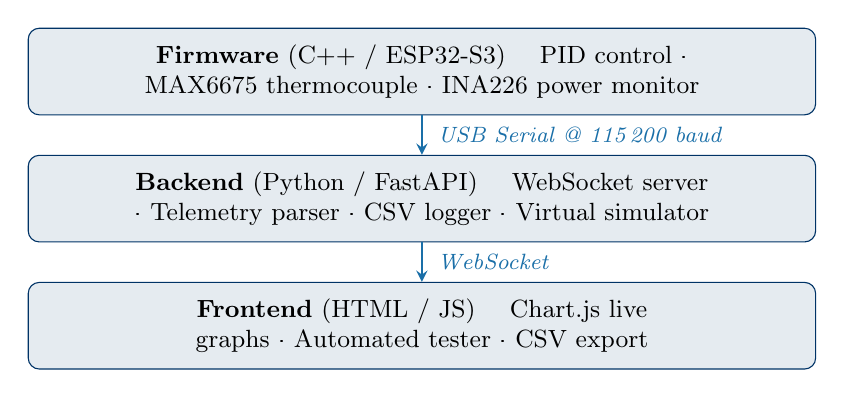
\begin{tikzpicture}[font=\small, node distance=0.6cm]
    \tikzstyle{tier}=[draw=hlblue, fill=hlblue!10, rounded corners,
                      minimum width=10cm, minimum height=1.1cm,
                      text width=9.5cm, align=center]
    \tikzstyle{arrow}=[draw=hllightblue, thick, ->, >=stealth]
    \tikzstyle{label}=[font=\footnotesize\itshape, text=hllightblue]

    \node[tier] (fw) {\textbf{Firmware} (C++ / ESP32-S3) \quad
                      PID control · MAX6675 thermocouple · INA226 power monitor};
    \node[tier, below=0.5cm of fw] (be)
                     {\textbf{Backend} (Python / FastAPI) \quad
                      WebSocket server · Telemetry parser · CSV logger · Virtual simulator};
    \node[tier, below=0.5cm of be] (fe)
                     {\textbf{Frontend} (HTML / JS) \quad
                      Chart.js live graphs · Automated tester · CSV export};

    \draw[arrow] (fw.south) -- node[label, right=2pt]{USB Serial @ 115\,200 baud} (be.north);
    \draw[arrow] (be.south) -- node[label, right=2pt]{WebSocket} (fe.north);
  \end{tikzpicture}
  \note{The whole system is split into three clear tiers, each talking to the next
  through a well-defined interface. At the bottom — closest to the hardware — is the
  firmware running on the ESP32-S3. It runs the PID loop, reads the sensors, and
  streams telemetry over USB serial at 115,200 baud. The key design decision here
  was to treat the firmware as a stable black box. I never changed it once it was
  validated. All user-facing features live in the two software tiers above.
  The backend is a Python FastAPI server that reads the serial port, parses the
  telemetry, and relays it to the browser over WebSocket. The frontend is a
  single HTML file with JavaScript — no build step, no dependencies, just open
  the file in a browser. I'll go much deeper into how these layers talk to each
  other in the software slides.}
\end{frame}

%% ---- SLIDE 6: Wind Tunnel ----------------------------------
\begin{frame}{Wind Tunnel Construction}
  \begin{columns}[T]
    \column{0.5\textwidth}
    \begin{itemize}
      \item Short rectangular enclosure — \textbf{chipboard panels}
      \item Fan at one end drives forced-convection airflow
      \item \textbf{Hexagonal honeycomb grid} immediately downstream of the fan
      \begin{itemize}
        \item Breaks up rotational vortex flow from the fan blades
        \item Produces a more \alert{uniform, laminar-like velocity profile} across the test section
        \item Critical for fair heatsink comparison: every sample sees the same airflow
      \end{itemize}
      \item Heater module sits at the centre of the test section
    \end{itemize}
    \column{0.47\textwidth}
    \centering
    \imgplaceholder[3.8cm]{Wind tunnel exterior\\— full view}\\[0.3em]
    \imgplaceholder[3.8cm]{Fan end with HEX grid\\close-up}
  \end{columns}
  \note{The wind tunnel is a simple chipboard box. The fan sits at one end, and a
  hexagonal honeycomb grid sits immediately behind it. The reason for the HEX grid
  is flow conditioning. A raw axial fan produces a swirling, non-uniform flow —
  the air spins as it comes off the blades. If you put a heatsink in that, one side
  sees more airflow than the other, and your measurement is not repeatable.
  The honeycomb cells break up that rotation and straighten the flow into a more
  uniform profile across the cross section. This is the same principle used in
  wind tunnels used for research and aerodynamic testing, just at a much smaller
  scale and lower budget. The result is that every heatsink you test sits in
  essentially the same airflow conditions — which is the whole point.}
\end{frame}

%% ---- SLIDE 7: Heater Module --------------------------------
\begin{frame}{The Heater Module}
  \begin{columns}[T]
    \column{0.52\textwidth}
    \textbf{Stack (bottom to top):}
    \begin{enumerate}
      \item Insulation material — prevents heat loss downward
      \item \textbf{Steel backing plate} — structural support
      \item \textbf{Ceramic PTC heater element} — the heat source
      \item \textbf{Copper spreader plate} — distributes heat uniformly
      \item Heatsink under test — clipped on with a wire retaining clip
    \end{enumerate}
    \vspace{0.4em}
    \textbf{Thermocouple:} inserted into a precision-drilled hole in the copper plate
    — tracks heatsink base temperature directly.\\[0.3em]
    \textbf{Built with:} Miquel Lladó i Tuñà (copper plate, steel backing, insulation)
    \column{0.45\textwidth}
    \centering
    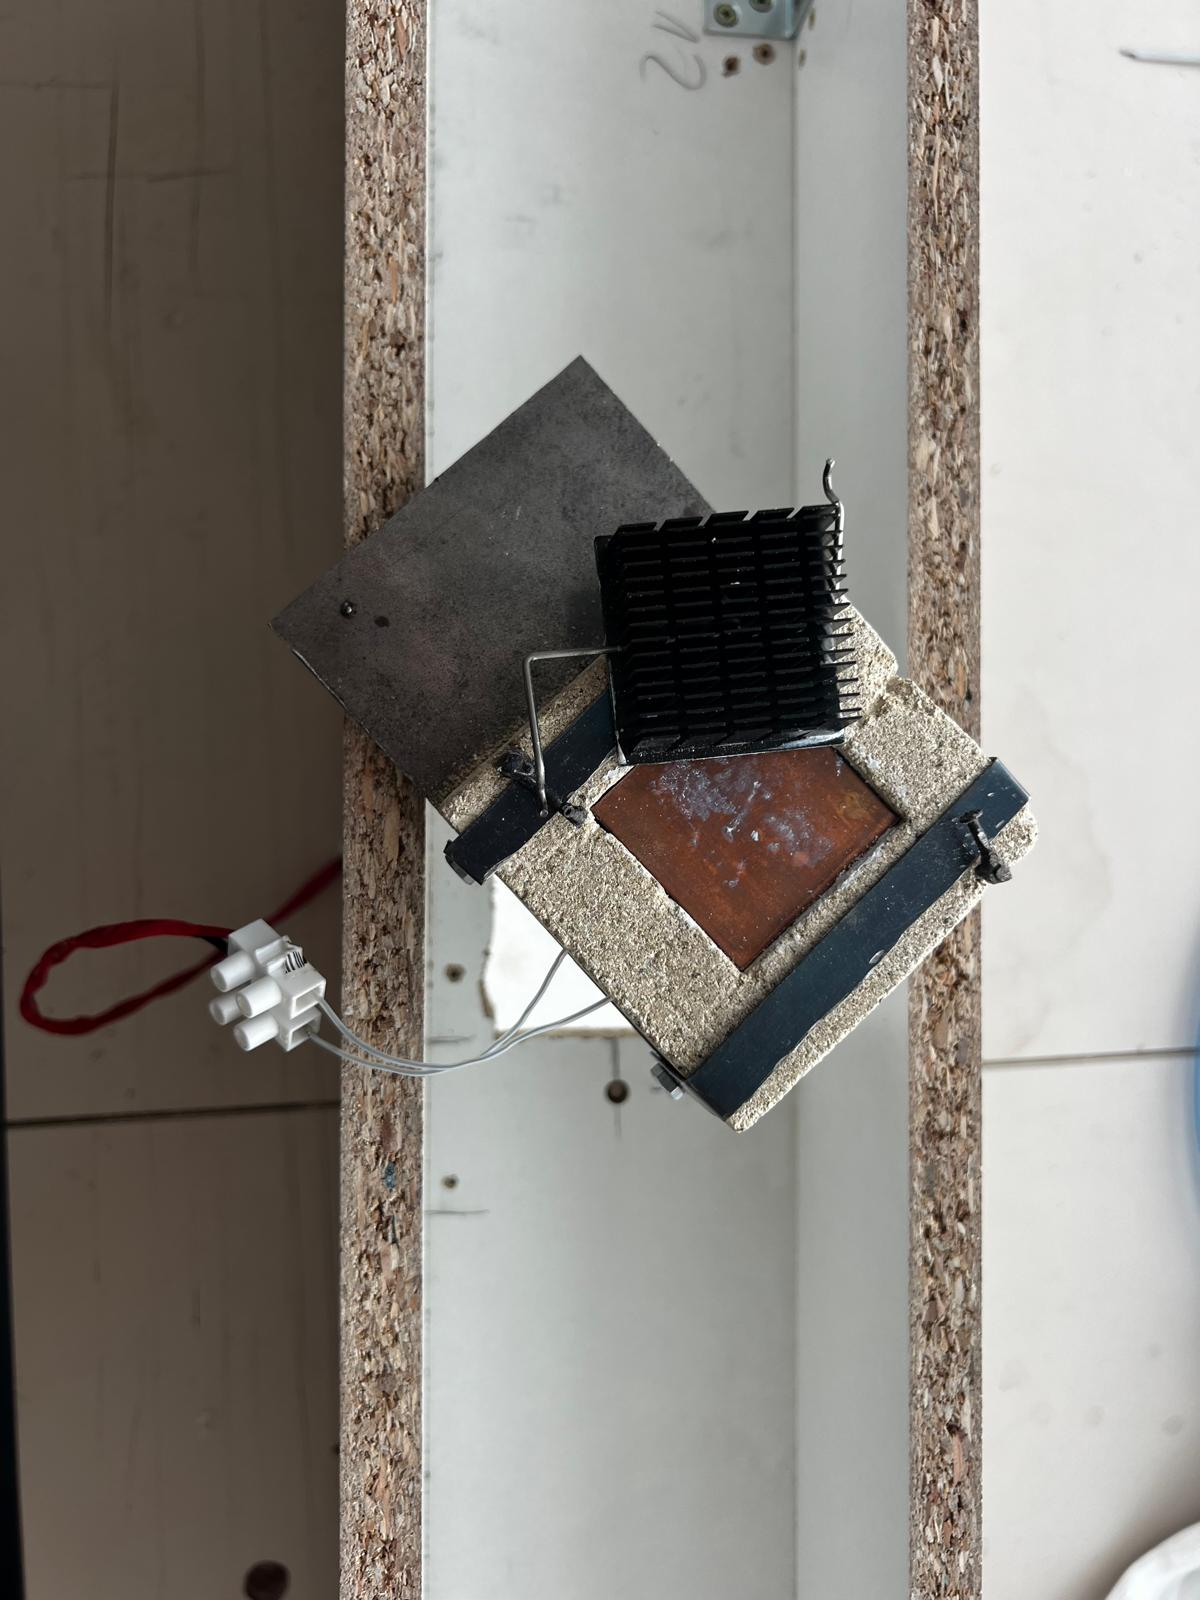
\includegraphics[width=\linewidth, height=3.6cm, keepaspectratio]{hw-01.jpeg}\\[0.3em]
    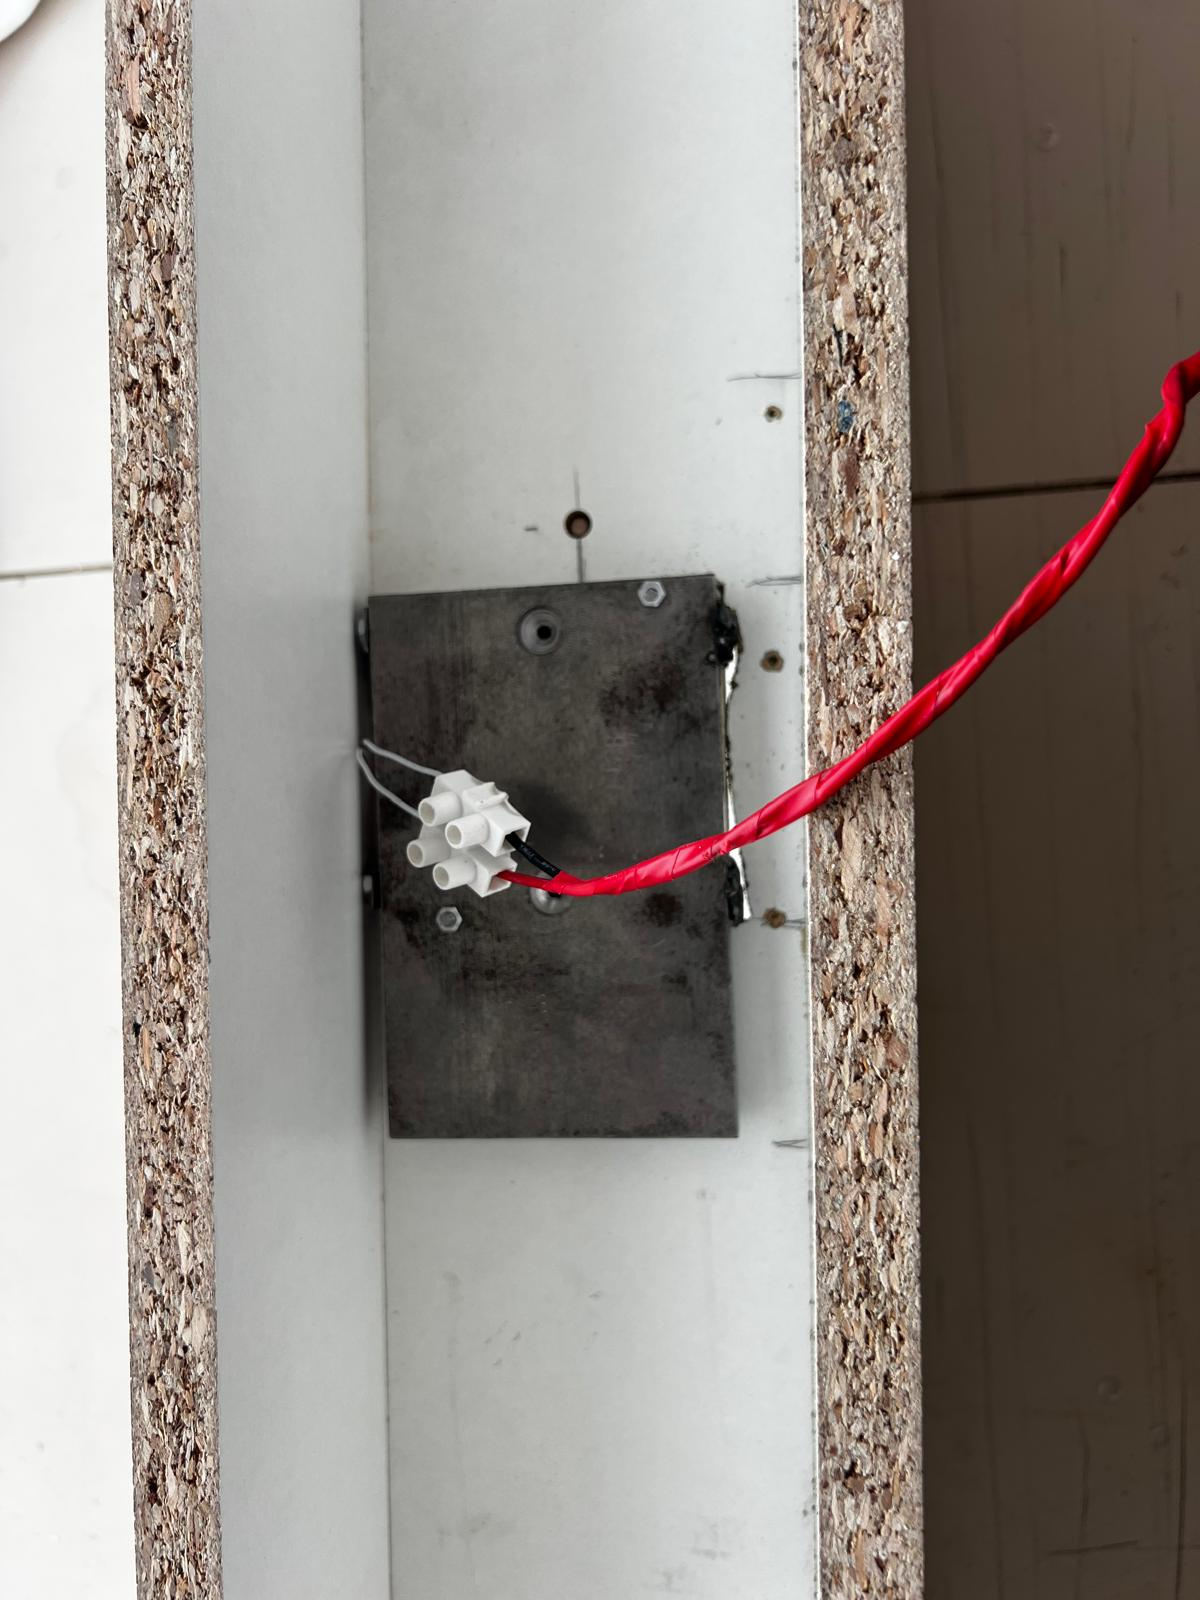
\includegraphics[width=\linewidth, height=3.6cm, keepaspectratio]{hw-03.jpeg}
  \end{columns}
  \note{The heater module is the heart of the physical platform. Working from the bottom:
  first a layer of insulation to stop heat escaping downward. Then a steel plate for
  structural rigidity. Then the ceramic PTC heater element — PTC stands for Positive
  Temperature Coefficient, which means its resistance rises with temperature, giving
  it a self-limiting property. On top of that is the copper spreader plate, which I
  want to emphasise: copper has excellent thermal conductivity, and the plate distributes
  the heat from the relatively small heater element uniformly across the larger base
  area that the heatsink will sit on. The heatsink clips on top with a spring-steel
  wire clip, so you can swap heatsinks quickly without tools. The thermocouple tip
  sits in a drilled hole in the copper — not on the heatsink surface — so the
  temperature we measure is the copper plate temperature, which is consistent across
  all tested heatsinks.}
\end{frame}

%% ---- SLIDE 8: Electronics & Sensors -----------------------
\begin{frame}{Electronics \& Sensors}
  \begin{columns}[T]
    \column{0.52\textwidth}
    \textbf{Key components:}
    \begin{itemize}
      \item \textbf{ESP32-S3 DevKit-C1} — microcontroller, runs firmware
      \item \textbf{MAX6675} — K-type thermocouple-to-digital converter (SPI)
      \item \textbf{INA226} — bi-directional current \& power monitor (I²C),\\
            shunt in series with heater → measures dissipated power directly
      \item \textbf{2× MOSFET modules} — switch heater (GPIO 4) and fan (GPIO 5)
      \item \textbf{Eventek KPS3010D} — 12 V / 10 A lab bench PSU
    \end{itemize}
    \vspace{0.3em}
    All electronics on a \textbf{perfboard dev board}, housed in the tunnel base.
    \column{0.45\textwidth}
    \centering
    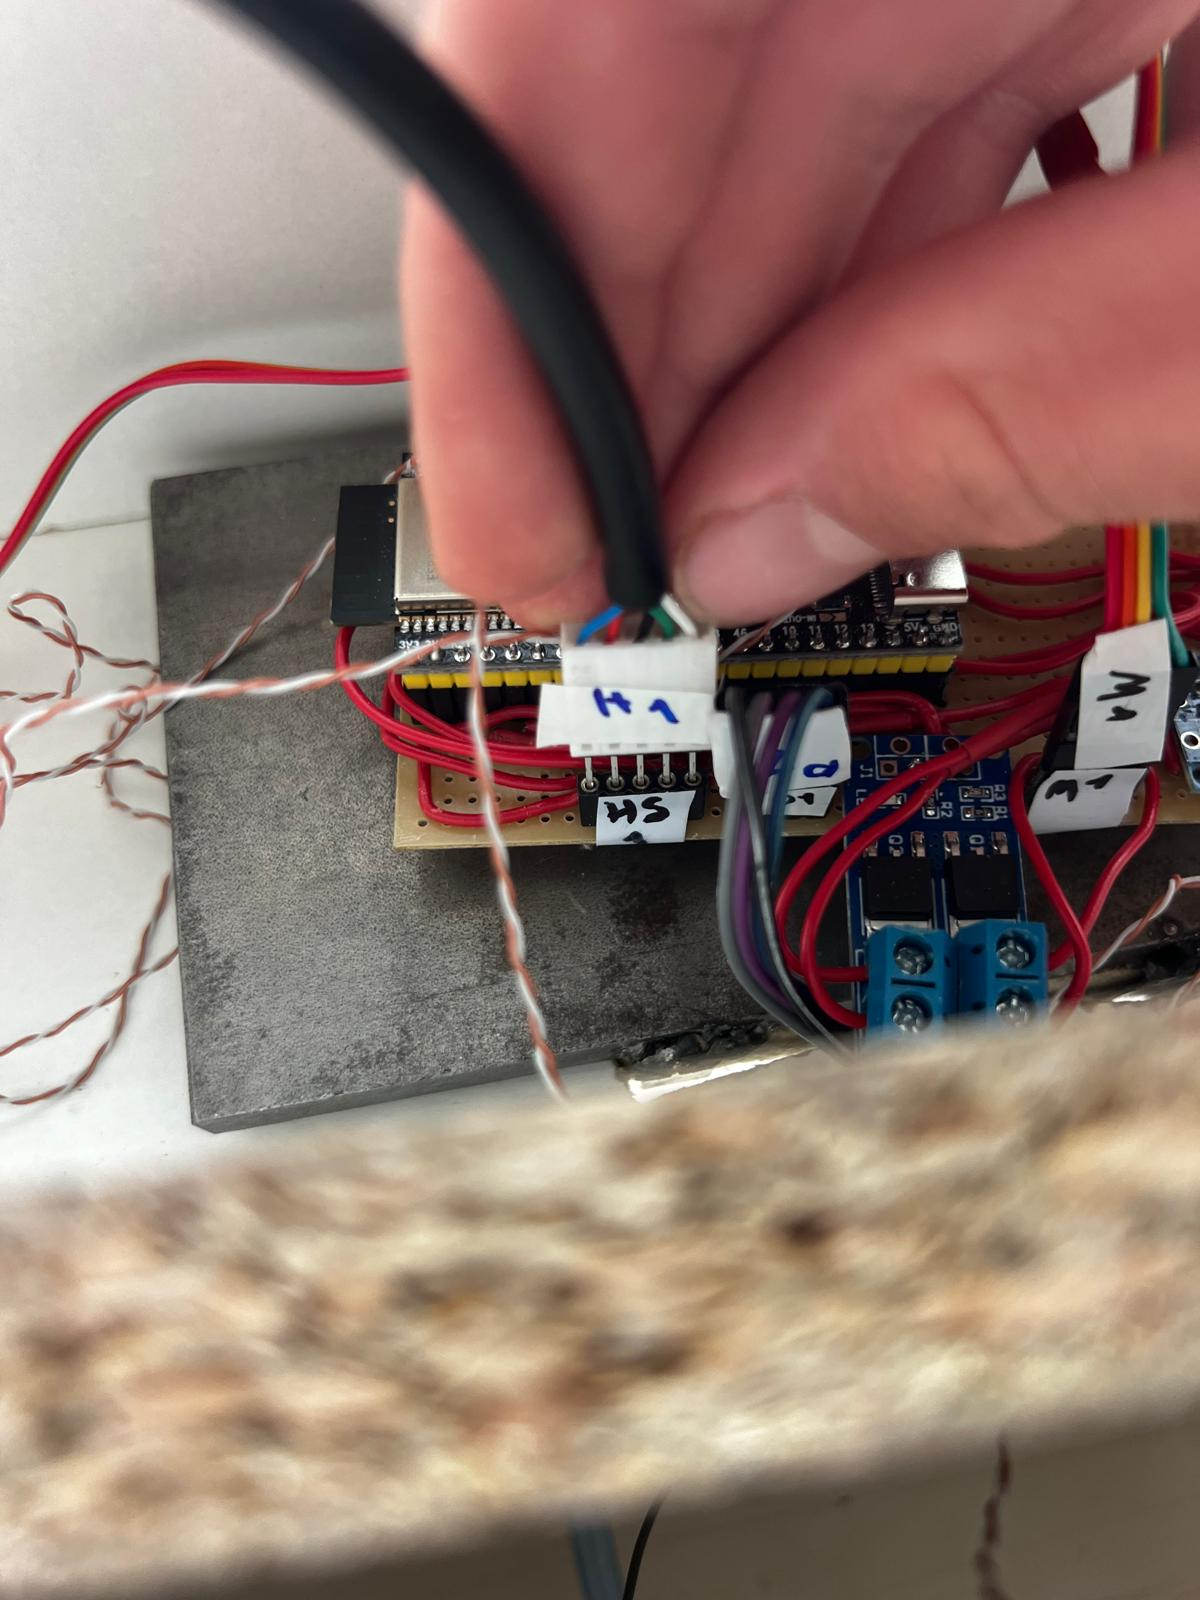
\includegraphics[width=\linewidth, height=3.6cm, keepaspectratio]{hw-17.jpeg}\\[0.3em]
    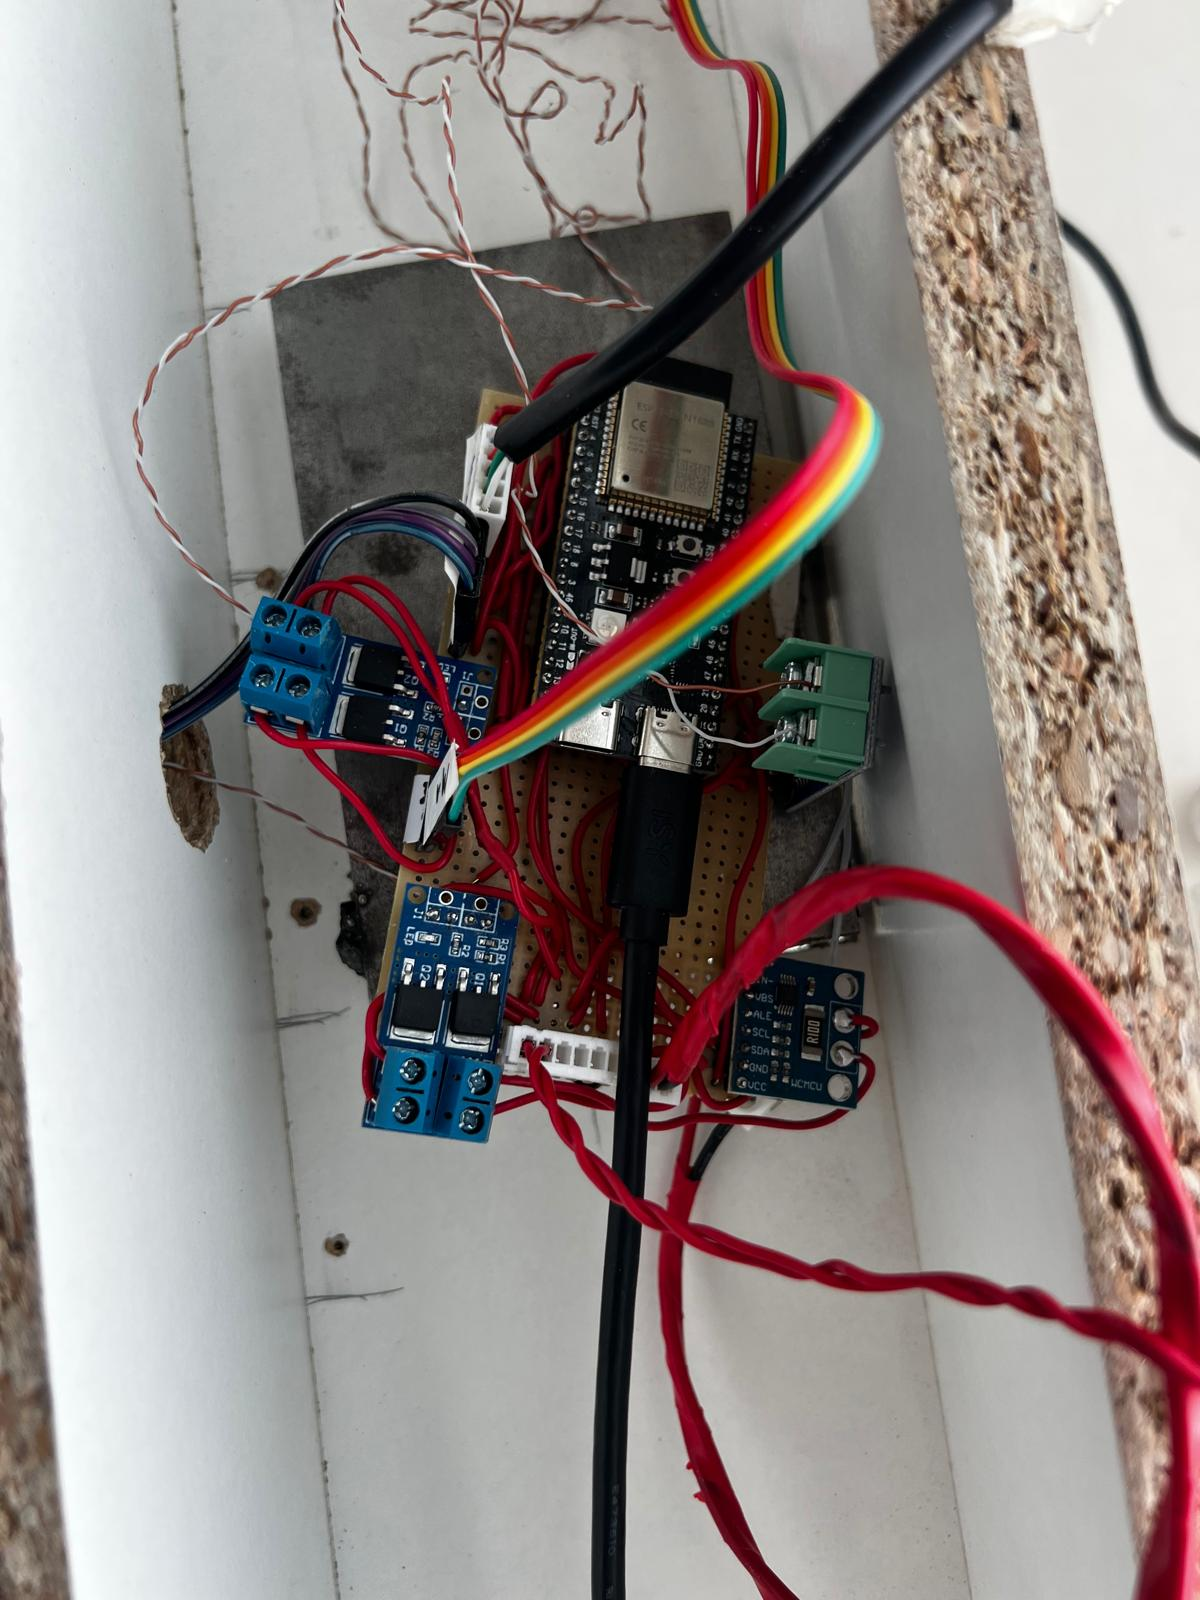
\includegraphics[width=\linewidth, height=3.6cm, keepaspectratio]{hw-22.jpeg}
  \end{columns}
  \note{Let me quickly run through the electronics. The ESP32-S3 is the brain —
  it reads sensors, runs the PID loop, and talks to the PC. The MAX6675 converts
  the thermocouple voltage to a digital reading over SPI — it also handles
  cold-junction compensation internally, which is important for thermocouple accuracy.
  The INA226 is particularly useful here: it measures both voltage and current
  simultaneously, so we get actual electrical power dissipated in the heater in watts
  — not estimated from a setpoint, but measured directly. The two MOSFETs are just
  electronic switches driven by PWM signals from the ESP32 — one for the heater,
  one for the fan. Everything sits on a handmade perfboard in a compartment under
  the tunnel. You can see the rainbow ribbon cable carrying the SPI thermocouple
  lines, and the red twisted cables for the 12 V heater power.}
\end{frame}

%% ---- SLIDE 9: Control Strategy: SMART Mode ----------------
\begin{frame}{Control Strategy: SMART Mode}
  \begin{columns}[T]
    \column{0.55\textwidth}
    \textbf{Three firmware control modes:} AUTO · MANUAL · \alert{SMART}\\[0.6em]
    \textbf{SMART mode — used for all automated tests:}
    \begin{enumerate}
      \item \textbf{PID drives} heater PWM toward set-point
      \item Temperature filtered by \textbf{EMA} (exponential moving average)\\
            + glitch rejection + stuck-sensor watchdog
      \item When stable within \alert{±\,0.5\,°C for 8 consecutive seconds}:\\
            enter \textbf{HOLD} — lock equilibrium PWM
      \item Backend independently checks \textbf{EqPWM convergence}\\
            (< 0.5 PWM units between frames) before recording
    \end{enumerate}
    \vspace{0.3em}
    \centering
    \setlength{\fboxsep}{6pt}
    \colorbox{hlblue!8}{%
      \small
      \texttt{PID (drive)} $\;\longrightarrow^{\pm0.5\,°C\;/\;8\,s}\;$ \texttt{HOLD (locked PWM)}
    }
    \column{0.42\textwidth}
    \vspace{0.5em}
    \textbf{Why lock the PWM?}\\
    At steady state, the equilibrium PWM directly tells us how much power the heater
    is delivering. Combined with the INA226 current reading, this gives us the
    dissipated power $P$ — which feeds directly into $R_{th} = \Delta T / P$.\\[0.6em]
    \textbf{Why dual-check?}\\
    Firmware stability band catches noise in the sensor. Backend EqPWM convergence
    catches slow drift that passes the firmware test but isn't truly settled.
  \end{columns}
  \note{SMART mode is the key control innovation in the firmware. It starts in PID
  mode — continuously adjusting heater power to drive the temperature toward the
  setpoint. Once the temperature stays within half a degree of the setpoint for
  8 consecutive seconds, it switches to HOLD: the PWM is frozen at its current
  value. This is important because a locked PWM means a stable, known power level —
  which is exactly what we need to compute thermal resistance. The EMA filter
  smooths the thermocouple reading to reduce cycle-to-cycle noise. There's also a
  second check on the backend side: the backend tracks the equilibrium PWM estimate
  and only records a data point when that estimate has also converged, meaning it
  changes by less than half a PWM unit between telemetry frames. This dual-check
  approach means we never record a point prematurely.}
\end{frame}

%% ---- SLIDE 10: Thermal Metric R_th -------------------------
\begin{frame}{Thermal Metric: Thermal Resistance $R_{th}$}
  \begin{columns}[T]
    \column{0.5\textwidth}
    \vspace{0.5em}
    \Large
    \[
      R_{th} = \frac{\Delta T}{P} \quad \left[\frac{{}^{\circ}\mathrm{C}}{\mathrm{W}}\right]
    \]
    \normalsize
    \vspace{0.3em}
    where $\Delta T = T_{heatsink} - T_{ambient}$\\
    and $P$ = electrical power dissipated by the heater [W]
    \vspace{0.8em}

    \begin{itemize}
      \item \textbf{Lower $R_{th}$} = heat removed more effectively = \alert{better heatsink}
      \item Measured at multiple set-points — $R_{th}$ should be \textbf{constant} (material/geometry property)
      \item Comparison is \textbf{fair} because airflow is identical for every heatsink tested
    \end{itemize}
    \column{0.47\textwidth}
    \vspace{0.5em}
    \textbf{Intuition:}\\[0.4em]
    A heatsink with \textbf{fins} has far more convective surface area than a plain block,
    even if the plain block is made of copper (higher conductivity). Under forced airflow,
    surface area dominates — so a finned aluminium heatsink typically outperforms a solid
    copper block.\\[0.6em]
    This is exactly what the results show.
  \end{columns}
  \note{The thermal metric is beautifully simple: temperature rise divided by power.
  If you put 10 watts into a heatsink and its temperature rises 30 degrees above ambient,
  the thermal resistance is 3 degrees per watt. A better heatsink — one that sheds heat
  more efficiently — rises less, so its $R_{th}$ is lower. We measure this at several different
  temperatures to confirm it's stable — $R_{th}$ is a property of the heatsink geometry and
  material, not of the operating point, so if our measurements are good, the values should
  be consistent across set-points. The comparison is fair because the wind tunnel runs at
  the same fan speed for every heatsink, so they all see the same airflow conditions.
  I want to quickly address the fins vs copper point, because it surprises people: copper
  has roughly twice the thermal conductivity of aluminium. But under forced airflow, what
  matters most is convective surface area — how much surface the air can actually touch.
  A finned aluminium heatsink has many times more surface area than a solid copper block
  of the same base footprint, so the fins win despite the material disadvantage.}
\end{frame}

%% ---- SLIDE 11: Software Data Flow --------------------------
\begin{frame}{Software Architecture: Data Flow}
  \centering
  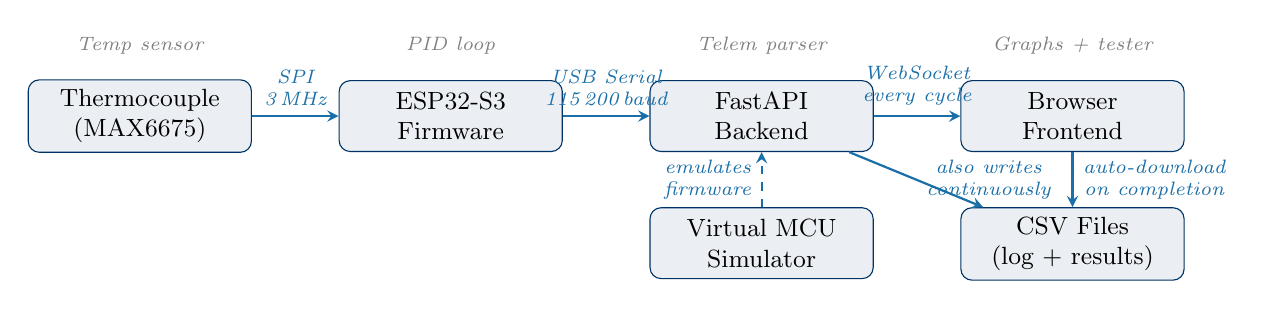
\begin{tikzpicture}[font=\small, node distance=0.45cm and 0.1cm]
    \tikzstyle{box}=[draw=hlblue, fill=hlblue!8, rounded corners,
                     minimum height=0.9cm, text width=2.6cm, align=center]
    \tikzstyle{arrow}=[draw=hllightblue, thick, ->, >=stealth]
    \tikzstyle{proto}=[font=\scriptsize\itshape, text=hllightblue, align=center]

    \node[box] (tc)  {Thermocouple\\(MAX6675)};
    \node[box, right=1.1cm of tc]  (fw)  {ESP32-S3\\Firmware};
    \node[box, right=1.1cm of fw]  (be)  {FastAPI\\Backend};
    \node[box, right=1.1cm of be]  (fe)  {Browser\\Frontend};
    \node[box, below=0.7cm of fe]  (csv) {CSV Files\\(log + results)};
    \node[box, below=0.7cm of be]  (vm)  {Virtual MCU\\Simulator};

    \draw[arrow] (tc) -- node[proto,above]{SPI\\3\,MHz} (fw);
    \draw[arrow] (fw) -- node[proto,above]{USB Serial\\115\,200\,baud} (be);
    \draw[arrow] (be) -- node[proto,above]{WebSocket\\every cycle} (fe);
    \draw[arrow] (fe) -- node[proto,right]{auto-download\\on completion} (csv);
    \draw[arrow] (be) -- node[proto,right]{also writes\\continuously} (csv);
    \draw[arrow, dashed] (vm) -- node[proto,left]{emulates\\firmware} (be);

    \node[above=0.2cm of tc, font=\scriptsize\itshape, text=gray]
          {Temp sensor};
    \node[above=0.2cm of fw, font=\scriptsize\itshape, text=gray]
          {PID loop};
    \node[above=0.2cm of be, font=\scriptsize\itshape, text=gray]
          {Telem parser};
    \node[above=0.2cm of fe, font=\scriptsize\itshape, text=gray]
          {Graphs + tester};
  \end{tikzpicture}
  \note{This is the full data pipeline from sensor to screen. Let me walk through
  it left to right. The thermocouple talks to the ESP32 over SPI — that's a fast
  synchronous bus, the reading takes a few microseconds each firmware cycle.
  The firmware runs the PID calculation, applies the EMA filter, and emits one
  telemetry line over USB serial at 115,200 baud — roughly every 100 milliseconds.
  The backend reads that serial stream continuously, parses each line with a single
  regular expression called TELEM\_RE, extracts all the fields, and immediately
  broadcasts a WebSocket message to every connected browser.
  The frontend receives that WebSocket message on every cycle and updates the live
  Chart.js graph and the sidebar readouts. It also runs the tester state machine —
  I'll explain that shortly. The backend writes every single telemetry frame to the
  raw log CSV as it arrives. The frontend writes the results CSV and triggers an
  automatic download when the test completes. The dashed box on the left is the
  virtual MCU simulator — it produces fake telemetry so you can run the entire
  workflow without a physical ESP32 attached.}
\end{frame}

%% ---- SLIDE 12: Backend Deep-Dive --------------------------
\begin{frame}{Backend: \texttt{server.py}}
  \begin{columns}[T]
    \column{0.5\textwidth}
    \textbf{Key responsibilities:}
    \begin{itemize}
      \item \textbf{\texttt{\_serial\_reader()}} — async loop, reads one line at a time from the COM port at 115,200 baud
      \item \textbf{\texttt{\_handle\_line()}} — applies \texttt{TELEM\_RE} (single regex) to extract all telemetry fields; calls \texttt{broadcast()}
      \item \textbf{\texttt{broadcast()}} — pushes a JSON \texttt{"telemetry"} message to every connected WebSocket client
      \item \textbf{\texttt{sendCmd()}} — sends \texttt{SET} / \texttt{GET} commands to the firmware
      \item \textbf{CSV logger} — appends each frame to the raw log; \texttt{CSV\_FIELDS} + \texttt{schema\_version}
    \end{itemize}
    \column{0.47\textwidth}
    \textbf{Virtual MCU Simulator:}\\
    Selecting the \texttt{VIRTUAL} port runs a software emulator that produces realistic telemetry — PID behaviour, equilibrium detection, ramp-up — with no hardware.\\[0.5em]
    \alert{Used to develop and debug the entire tester workflow before the hardware existed.}\\[0.5em]
    \textbf{WebSocket messages} (type field):\\
    \texttt{"telemetry"} · \texttt{"ports"} · \texttt{"connected"}\\
    \texttt{"disconnected"} · \texttt{"error"}
  \end{columns}
  \note{The backend is a single Python file — server.py — built with FastAPI and the
  asyncio event loop. The serial reader runs as a continuous async coroutine, reading
  one text line at a time from the serial port. Each line is handed to handle\_line,
  which applies the TELEM\_RE regular expression — a single, comprehensive regex with
  named capture groups for every telemetry field. This is deliberately a single regex
  rather than multiple passes, so there's one place to maintain when the firmware
  adds a new field. The broadcast function then serialises all the extracted fields
  into a JSON message and sends it to every connected browser over WebSocket. It
  also writes the frame to the raw log CSV. The sendCmd function queues serial
  commands — things like SET SP 50 to set a 50-degree setpoint, or SET RUN OFF
  to cut heater power. The virtual simulator was incredibly valuable: it let me
  write and debug the entire automated test workflow, the equilibrium detection,
  the CSV export, and the safety shutdown, all without needing the physical hardware
  to be ready. Every safety mechanism was tested in simulation before I ever
  energised the heater.}
\end{frame}

%% ---- SLIDE 13: Frontend Deep-Dive -------------------------
\begin{frame}{Frontend: \texttt{index.html}}
  \begin{columns}[T]
    \column{0.52\textwidth}
    \textbf{Single file — all HTML, CSS, and JavaScript}\\
    (No build step, no Node.js, no internet required)\\[0.5em]
    \textbf{WebSocket \texttt{onmessage} handler:}
    \begin{itemize}
      \item Receives \texttt{"telemetry"} every firmware cycle
      \item Updates \textbf{Chart.js} live temperature trace
      \item Updates sidebar readouts (temp, power, PWM, fan speed…)
    \end{itemize}
    \vspace{0.4em}
    \textbf{Tester state machine (JavaScript):}
    \begin{itemize}
      \item Steps through the programmed set-points
      \item Watches \texttt{eq\_pwm} convergence on each telemetry frame
      \item When converged: records a result row
      \item Advances to next set-point — or ends test
      \item Auto-downloads results CSV on completion
    \end{itemize}
    \column{0.45\textwidth}
    \centering
    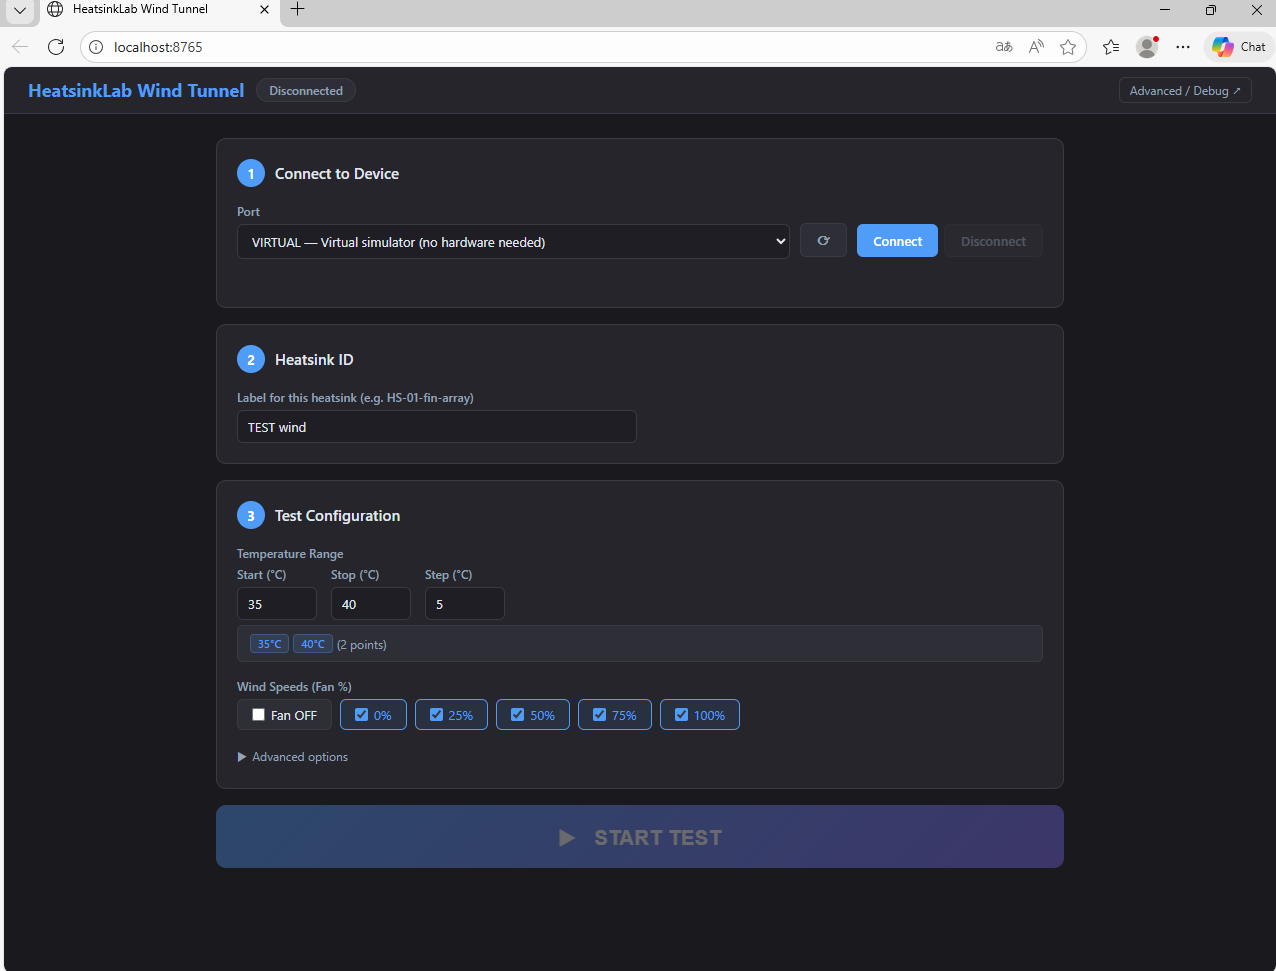
\includegraphics[width=\linewidth, height=3.6cm, keepaspectratio]{sw-03.png}\\[0.3em]
    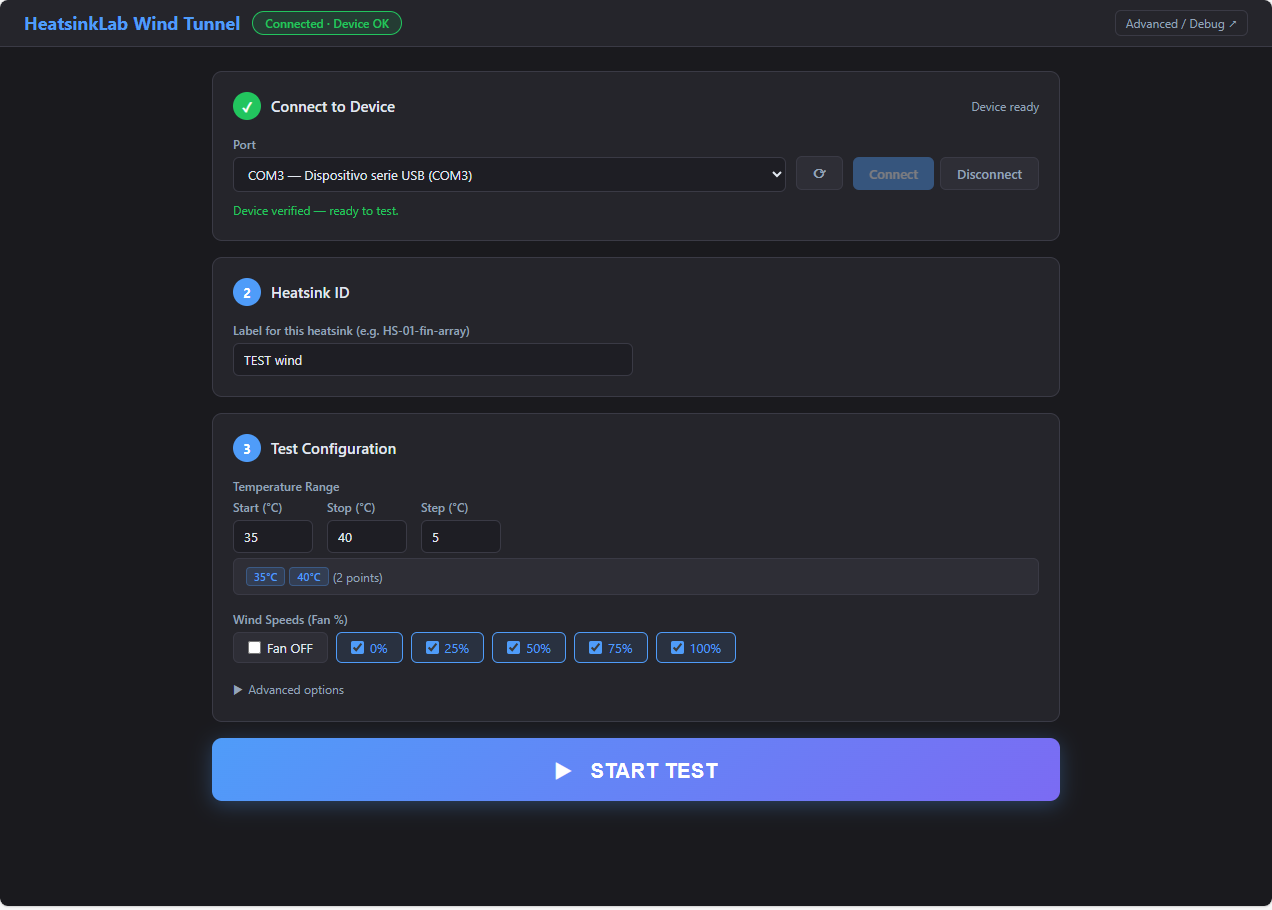
\includegraphics[width=\linewidth, height=3.6cm, keepaspectratio]{sw-07.png}
  \end{columns}
  \note{The frontend is intentionally a single HTML file with everything inline —
  HTML structure, CSS styles, and all the JavaScript logic. This is a deliberate
  design choice for the lab deployment: you can copy it to any machine with Python
  installed and it just works. No package manager, no build step, no internet.
  The WebSocket message handler receives the telemetry JSON on every firmware cycle
  and does two things: updates the live Chart.js graph with the new temperature
  point, and refreshes all the sidebar readout fields. The tester state machine is
  the key piece of automation. It lives in JavaScript and it watches the incoming
  telemetry. When it's waiting for equilibrium, it checks whether the eq\_pwm field
  — the equilibrium PWM estimate from the firmware — has converged: changed by less
  than 0.5 units between frames. When that condition is true, it records the current
  temperature, power, and other readings as one row in the results table, then either
  commands the next setpoint or — if that was the last one — triggers the shutdown
  sequence and automatically downloads the CSV file. The student never has to click
  Download.}
\end{frame}

%% ---- SLIDE 14: The Automated Workflow ---------------------
\begin{frame}{The Automated Workflow}
  \begin{columns}[T]
    \column{0.48\textwidth}
    \textbf{Student steps (all of them):}
    \begin{enumerate}
      \item Plug in ESP32 via USB
      \item Double-click \textit{HEATSINK TESTER} shortcut
      \item Select COM port → click Connect
      \item Type heatsink ID (e.g.\ \texttt{HS-01-fin-array})
      \item Press \alert{Start Test}
      \item \textbf{Wait} — system steps through all temperatures automatically
      \item Results CSV downloads automatically when complete
      \item Swap heatsink → repeat from step 4
    \end{enumerate}
    \vspace{0.2em}
    \textit{Students never need to know what PID is.}
    \column{0.5\textwidth}
    \centering
    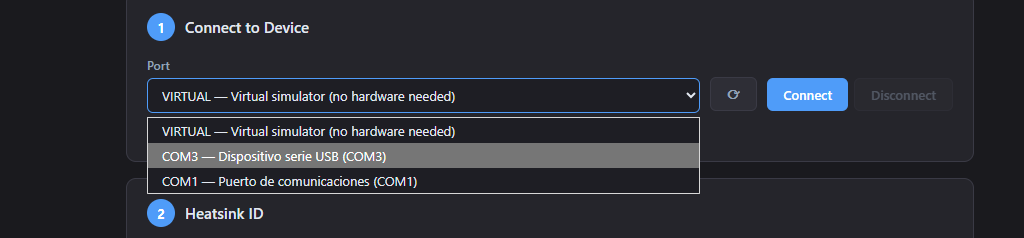
\includegraphics[width=0.48\linewidth, height=3cm, keepaspectratio]{sw-05.png}\hfill
    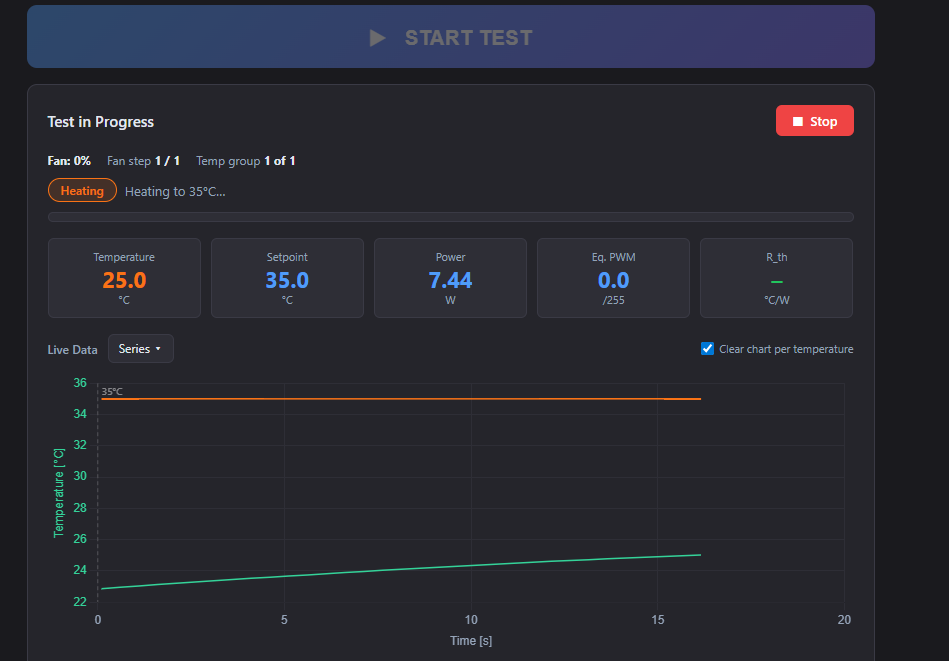
\includegraphics[width=0.48\linewidth, height=3cm, keepaspectratio]{sw-08.png}\\[0.3em]
    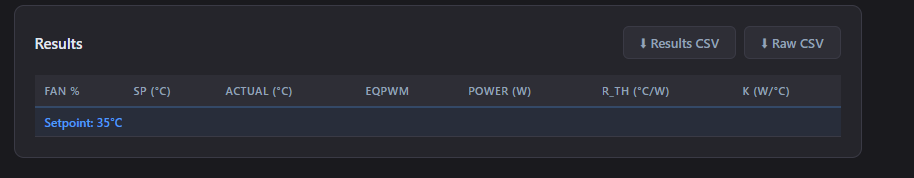
\includegraphics[width=\linewidth, height=3cm, keepaspectratio]{sw-09.png}
  \end{columns}
  \note{This slide is really the point of the whole project. Eight steps, but the
  student only actively does five of them — the rest are automatic. The connection
  wizard shows a numbered layout so even a student who has never used lab software
  knows what to do next. Once Start Test is pressed, the system drives the heater
  to the first setpoint, waits for equilibrium in SMART mode, records the data point,
  advances to the next setpoint, and repeats until all setpoints are done. Then it
  shuts off the heater, runs a cool-down, and automatically downloads the CSV.
  The student doesn't need to watch the screen. They can step away, come back when
  the test is done, and their results file is already on the desktop. You can see
  in the screenshots: the port selector on the top left, the live temperature chart
  in the middle, and the results panel with download buttons at the bottom right.}
\end{frame}

%% ---- SLIDE 15: Results ------------------------------------
\begin{frame}{Results: $R_{th}$ Comparison}
  \begin{columns}[T]
    \column{0.5\textwidth}
    \vspace{0.3em}
    \small
    \begin{tabularx}{\linewidth}{@{}Xrrrr@{}}
      \toprule
      Heatsink & SP\,(°C) & P\,(W) & $R_{th}$\,(°C/W) \\
      \midrule
      HS-01 fin-array & 40 & 7.6  & 2.38 \\
      HS-01 fin-array & 50 & 11.6 & 2.42 \\
      HS-01 fin-array & 60 & 15.9 & 2.38 \\
      \midrule
      HS-02 copper block & 40 & 4.4  & 4.05 \\
      HS-02 copper block & 50 & 7.0  & 3.99 \\
      HS-02 copper block & 60 & 9.5  & 3.97 \\
      \bottomrule
    \end{tabularx}
    \vspace{0.3em}
    \footnotesize\textit{Representative values — illustrate output format.}
    \column{0.47\textwidth}
    \vspace{0.3em}
    \textbf{Key observations:}
    \begin{itemize}
      \item $R_{th}$ is \alert{consistent across set-points} for each heatsink — confirms steady-state measurement quality
      \item \textbf{Finned aluminium (HS-01) outperforms solid copper (HS-02)} despite copper's higher conductivity: fins provide far more convective surface area
      \item HS-01 needs \textbf{more power} to hold the same temperature — more heat is being removed by the airflow, so the heater has to work harder
      \item Platform \alert{clearly distinguishes} the two samples: 2.4 vs 4.0\,°C/W
    \end{itemize}
  \end{columns}
  \note{These are representative values that illustrate the format of the output.
  The first thing to notice is that $R_{th}$ is consistent across set-points for each
  heatsink — 2.38, 2.42, 2.38 for the fin array. That consistency is exactly what
  we expect from theory, and it tells us the measurement is working correctly.
  The second observation is that the finned aluminium heatsink is substantially
  better than the solid copper block — 2.4 versus 4.0 degrees per watt, a factor
  of 1.7. Despite copper's higher thermal conductivity, the fins create so much
  more surface area for the air to contact that they win decisively. Notice also
  that HS-01 requires more heater power for the same temperature — because it's
  shedding more heat to the airflow, the heater has to work harder to maintain
  the setpoint. That's a really clean physical consistency check on the data.
  The platform answered RQ4: yes, it meaningfully distinguishes heatsinks.}
\end{frame}

%% ---- SLIDE 16: Safety -------------------------------------
\begin{frame}{Safety: Heater Shutdown}
  \begin{columns}[T]
    \column{0.55\textwidth}
    \textbf{Three tested termination paths — all verified:}
    \begin{enumerate}
      \item \textbf{Normal test completion}\\
            Backend sends \texttt{SET RUN OFF} automatically after the last set-point.
            GUI displays \textit{"Test complete — heater off"}.
      \vspace{0.4em}
      \item \textbf{Manual Stop button}\\
            Immediately sends \texttt{SET RUN OFF}.
            Heater power drops to zero within one firmware cycle.
      \vspace{0.4em}
      \item \textbf{Browser close / network disconnect}\\
            Backend detects WebSocket disconnection and sends \texttt{SET RUN OFF} as a fallback.
    \end{enumerate}
    \vspace{0.4em}
    \alert{In all three cases: INA226 power reading returned to zero.}
    \column{0.42\textwidth}
    \vspace{0.5em}
    \textbf{Why this matters:}\\[0.3em]
    A heater left on unattended in a lab is a genuine fire and burn risk.
    Requiring a student to manually cut power after the test means relying on
    a human action that can be forgotten.\\[0.5em]
    \textbf{Automatic shutdown on every exit path} removes that dependency entirely.\\[0.5em]
    Additionally: a 60-second cool-down at low fan speed runs before the fan stops,
    reducing thermal stress on components.
  \end{columns}
  \note{Safety was requirement R5 and I treated it as P0 — the highest priority.
  A live heater element in a teaching lab is a real hazard. I tested three ways the
  test can end. First, the happy path: test completes normally, backend sends
  SET RUN OFF, the GUI confirms the heater is off. Second, mid-run stop: pressing
  the Stop button sends the command immediately, and the INA226 current reading
  drops to zero within one 100-millisecond firmware cycle. Third, the browser just
  gets closed or the network drops — this is the failure mode that's easiest to
  miss. The backend detects the WebSocket disconnection event and sends SET RUN OFF
  as a fallback within a second or two. In all three cases I confirmed with the
  INA226 that heater power actually went to zero — not just that the command was
  sent. After the shutdown, there's a 60-second cool-down period where the fan
  stays on at low speed, which protects the heater element and the copper plate
  from thermal shock.}
\end{frame}

%% ---- SLIDE 17: Limitations & Future Work ------------------
\begin{frame}{Limitations \& Future Work}
  \begin{columns}[T]
    \column{0.5\textwidth}
    \textbf{Current limitations:}
    \begin{itemize}
      \item \textbf{Airspeed commanded, not measured} — fan \% assumes reproducible fan curve; real m/s unknown
      \item \textbf{No independent hardware safety watchdog} — safety relies on firmware + backend logic; a separate MCU with its own power cut would be more robust
      \item \textbf{Single thermocouple} — no independent ambient sensor; T\_amb estimated manually
      \item \textbf{No formal repeatability study} — functional validation only; uncertainty budget not quantified
    \end{itemize}
    \column{0.47\textwidth}
    \textbf{Highest-priority next steps:}
    \begin{enumerate}
      \item Wire the \textbf{anemometer} and \textbf{SDP510 pressure sensor} — already provisioned in the telemetry schema and CSV; enables closed-loop airspeed control
      \item Add an \textbf{independent hardware watchdog MCU} with a power-cut relay
      \item Run a structured \textbf{repeatability study} on reference heatsinks
      \item Record \textbf{ambient temperature and humidity} per run (EZO-HUM already wired)
      \item Packaged \textbf{one-click installer} for lab deployment
    \end{enumerate}
  \end{columns}
  \note{Every system has limitations and this one is no different. The most significant
  technical gap is that airspeed is not measured — we set the fan to a percentage and
  assume that's reproducible. For comparison between sessions or between setups, you
  really want a measured air velocity. The good news is that the SDP510 differential
  pressure sensor is already physically installed and the data schema already has
  placeholder columns for it — wiring it up and writing the parser update is the
  next concrete step. The hardware safety watchdog is the other important gap: right
  now if the ESP32 firmware crashes or hangs, there's nothing to cut the heater power.
  A small second microcontroller with a watchdog timer and a relay is the correct
  fix. For future work, the repeatability study is important for any real scientific
  use of the platform — we'd need to quantify how much the $R_{th}$ varies between
  repeated tests of the same heatsink under the same conditions.}
\end{frame}

%% ---- SLIDE 18: Conclusion ----------------------------------
\begin{frame}{Conclusion}
  \begin{columns}[T]
    \column{0.55\textwidth}
    \textbf{All four research questions answered:}\\[0.3em]
    \begin{tabular}{@{}ll@{}}
      \textcolor{green!60!black}{\textbf{RQ1}} & PID + EMA: stable within ±\,0.5\,°C \\[0.2em]
      \textcolor{green!60!black}{\textbf{RQ2}} & Dual-check equilibrium detection: reliable \\[0.2em]
      \textcolor{green!60!black}{\textbf{RQ3}} & One button; shutdown on all exit paths \\[0.2em]
      \textcolor{green!60!black}{\textbf{RQ4}} & Platform distinguishes heatsinks clearly \\
    \end{tabular}
    \vspace{0.6em}
    \textbf{Key contributions:}
    \begin{itemize}
      \item Robust, safe, genuinely usable lab automation system
      \item \textbf{Software-first architecture}: firmware locked, all features in backend + frontend — rapid iteration, hardware unchanged from first prototype to final build
      \item Any engineering student can characterise a heatsink \alert{without knowing what PID is}
    \end{itemize}
    \column{0.42\textwidth}
    \centering
    \imgplaceholder[5.5cm]{Complete assembled system\\on the lab bench}
    \vspace{0.5em}
    \small\textit{Thank you.\\Questions?}
  \end{columns}
  \note{To close: I set out to build a system where a student could characterise a
  heatsink with a single button press, with the heater shutting off automatically.
  I achieved that. All four research questions have a positive answer. The PID loop
  is stable enough, equilibrium detection is reliable, the workflow is one button,
  and the platform clearly distinguishes heatsinks with different thermal properties.
  The key architectural decision — treating the firmware as a locked black box and
  putting everything student-facing in the software — meant I could develop, debug,
  and iterate quickly, and the safety-critical control loop never needed to change.
  The platform is usable by students who have never heard of PID, don't know what
  a COM port is, and have no data acquisition background. That was the goal from
  day one, and the system delivers it. I'm happy to take questions — either on the
  hardware design, the software architecture, the control strategy, or the results.}
\end{frame}

%% ============================================================
\end{document}
